\documentclass{article}
\usepackage{graphicx}
\usepackage{enumerate}
\usepackage{amsmath}
\usepackage{amsthm}
\usepackage{amsfonts}
\usepackage{hyperref}

\usepackage{amssymb}

\usepackage{amsmath}  

\usepackage{algorithm}  
\usepackage[noend]{algpseudocode}
\usepackage{algorithmicx,algorithm}

\usepackage{algpseudocode}  
\usepackage{amsmath}  
\renewcommand{\algorithmicrequire}{\textbf{Input:}}  % Use Input in the format of Algorithm  
\renewcommand{\algorithmicensure}{\textbf{Output:}} % Use Output in the format of Algorithm    
\usepackage{listings}
\usepackage{url}

\usepackage{etoolbox}
\newtoggle{solution}
\toggletrue{solution}
%\togglefalse{solution}
\usepackage{color}
\newcommand{\solution}[2][0pt]{\iftoggle{solution}{\smallskip{\color{red}{\flushleft\textbf{Solution}:}\par#2}}{\vspace*{#1}}}

\renewcommand{\baselinestretch}{1.2}%Adjust Line Spacing
%\geometry{left=2.0cm,right=2.0cm,top=2.0cm,bottom=2.0cm}% Adjust Margins of the File

% Create horizontal rule command with an argument of height
\newcommand{\horrule}[1]{\rule{\linewidth}{#1}}
% Set the title here
\title{
    \normalfont \normalsize
    \textsc{ShanghaiTech University} \\ [25pt]
    \horrule{0.5pt} \\[0.4cm] % Thin top horizontal rule
    \huge CS240 Algorithm Design and Analysis \\ % The assignment title
    \LARGE Fall 2022\\
    \LARGE Problem Set 4\\
    \horrule{2pt} \\[0.5cm] % Thick bottom horizontal rule
}
% wrong usage of \author, never mind
\author{Dai ZiJia 2022233158}
\date{Due: 23:59, Dec. 18, 2022}

% Add the support for auto numbering
% use \problem{title} or \problem[number]{title} to add a new problem
% also \subproblem is supported, just use it like \subsection
\newcounter{ProblemCounter}
\newcounter{oldvalue}
\newcommand{\problem}[2][-1]{
	\setcounter{oldvalue}{\value{secnumdepth}}
	\setcounter{secnumdepth}{0}
	\ifnum#1>0
		\setcounter{ProblemCounter}{#1}
	\else
		\stepcounter{ProblemCounter}
	\fi
	\section{Problem \arabic{ProblemCounter}: #2}
	\setcounter{secnumdepth}{\value{oldvalue}}
}
\newcommand{\subproblem}[1]{
	\setcounter{oldvalue}{\value{section}}
	\setcounter{section}{\value{ProblemCounter}}
	\subsection{#1}
	\setcounter{section}{\value{oldvalue}}
}

\begin{document}
\maketitle
\vspace{3ex}

\begin{enumerate}
%\item Please write your solutions in English. 
\item Submit your solutions to Gradescope (www.gradescope.com).
\item In ``Account Settings'' of Gradescope, set your FULL NAME to your Chinese name and enter your STUDENT ID correctly. 
\item If you want to submit a handwritten version, scan it clearly. Camscanner is recommended. 
\item When submitting your homework, match each of your solution to the corresponding problem number. 
%\item Violations to any of above may result in some penalty on your score. 
\end{enumerate}

\newpage
\problem{}
Run the Ford-Fulkerson algorithm on the flow network in the figure below, and
show the residual network after each flow augmentation. For each iteration, pick
the augmenting path that is lexicographically smallest. (e.g., if you have two
augmenting path 1 $\rightarrow$ 3 $\rightarrow$ t and 1 $\rightarrow$ 4 $\rightarrow$ t, then you should choose 1 $\rightarrow$ 3 $\rightarrow$ t,
which is lexicographically smaller than 1 $\rightarrow$ 4 $\rightarrow$ t)


\begin{figure}[htbp]
    \centering
    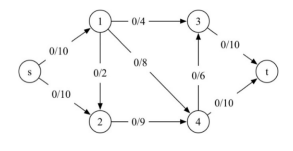
\includegraphics{HW2/1.png}
    \end{figure} 

Result as the following:
\begin{figure}[htbp]
\begin{center}	
	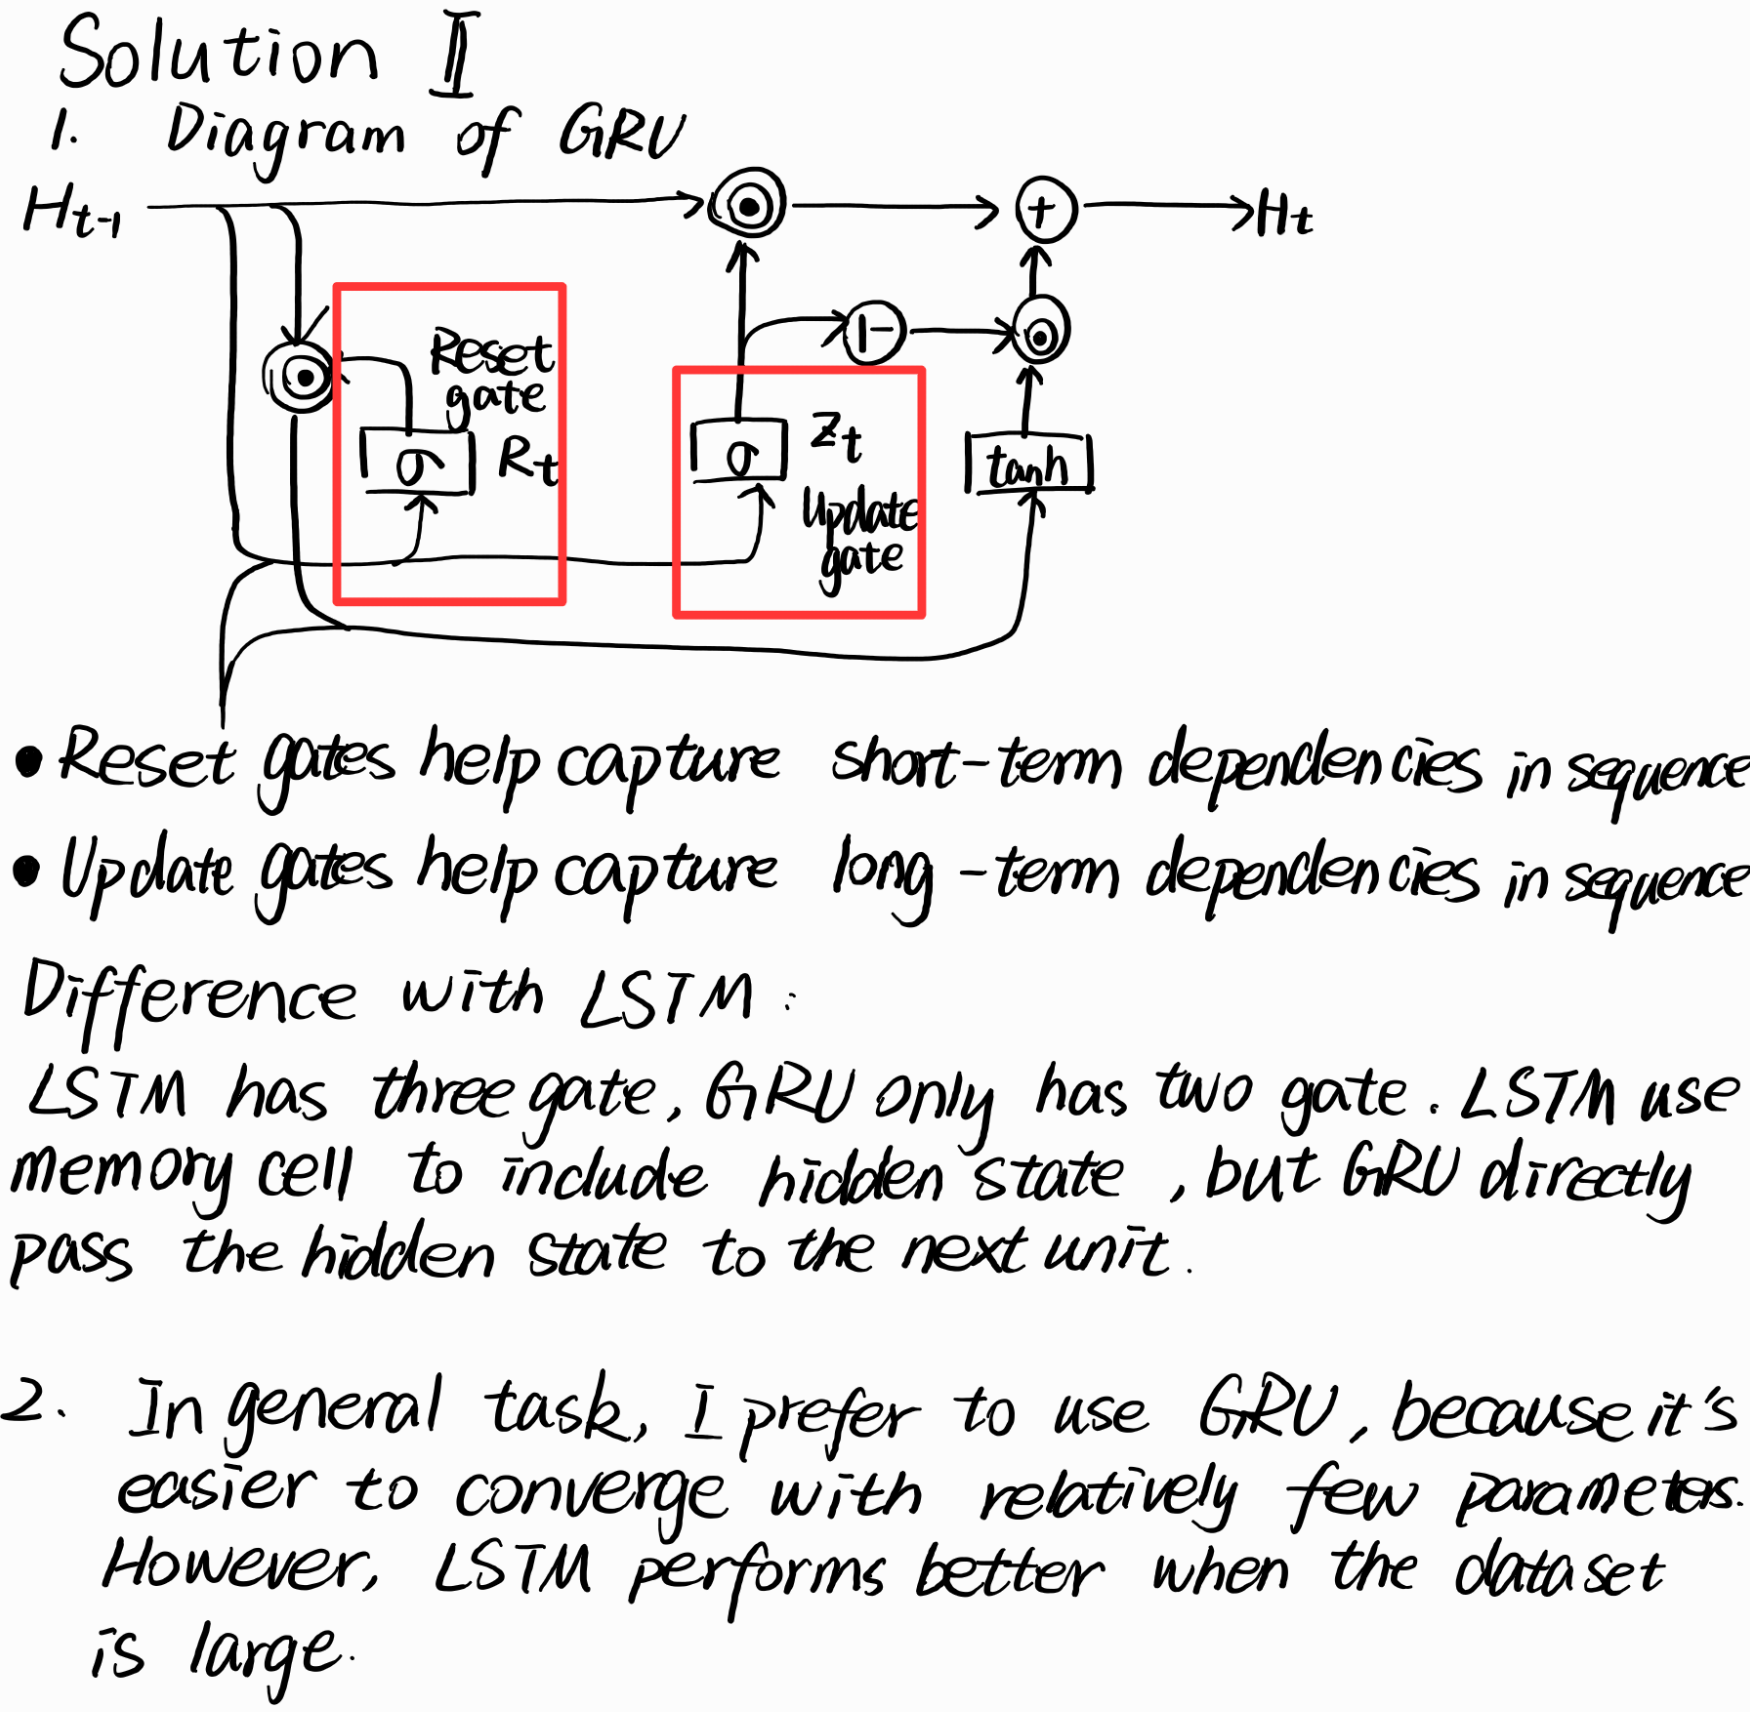
\includegraphics[width=1\textwidth]{HW2/2.png}
\end{center}
\end{figure} 


\newpage
\problem{}
Give the time complexity of the following code and explain the reason.
\begin{enumerate}[(1)]
	\item 
	
	\begin{lstlisting}
    for ( i=1; i < n; i *= 2 ) {
        for ( j = n; j > 0; j /= 2 ) {
            for ( k = j; k <= n; k += 2 ) {
                res += (i * j + j * k );
            }
        }
    }
    \end{lstlisting}
	
	\item 
	\begin{lstlisting}
    for ( i = n; i > 0; i -= 1 ) {
        for ( j = 1; j < n; j *= 2 ) {
            for ( k = 0; k < j; k += 1 ) {
                res += (i * j + j * k );
            }
        }
    }

\end{lstlisting}
\end{enumerate}

 
\solution{
\begin{enumerate}[(a)]
	\item 
	For i-loop is $O(logn)$, for j-loop is $O(logn)$, for k-loop is $O(n)$, so the total complexity is $O(nlog^2n)$.
	\item
	For i-loop is $O(n)$, for jk-loop is $O(n)$, because
	$$1 + 2 + 4 +...+ \frac{n}{2} = \frac{2(1-2^{logn})}{1-2} = 2n$$.
	So the total complexity is $O(n^2)$.
\end{enumerate}
}


\newpage
\problem{}
Suppose to perform a sequence of $n$ operations on a data structure. The $i$-th operation costs $i$ if $i$ is an exact power of 2, otherwise $i$-th operation costs 1.  
\newline
a) Using  accounting method to determine the amortized cost per operation.
\newline
b) Using  potential  method to determine the amortized cost per operation.

\solution{
\textbf{Accounting method:}
%The $i$-th operation costs $O(i)$ if $i$ is an exact power of 2, otherwise $i$-th operation costs $O(1)$. The %$n$ operations will cost:
%$$1+2+1+4+1+1+8+\cdots = n+(1+2+4+\cdots +\log n)-\log n$$
%$$=n+\frac{1\cdot(1-2^{\log (n-1)})}{1-2}=n+n-1-1 = 2n-2=O(2n)=O(n)$$
%It cost $O(n)$ in $n$ operations, so each operation cost $O(1)$.
We let $c'_i$ be the charge for the i-th operation, where $c_i$ is the true cost and $b_i$ is the balance after the i-th operation. We can set $c'_i=3$ for each operation cost. In 10 times iterations they appears to be:
\begin{table}[h!]
	\centering
	\begin{tabular}{lllllllllll}
		$i$    & 1 & 2 & 3 & 4 & 5 & 6 & 7  & 8 & 9 & 10 \\
		$c_i$  & 1 & 2 & 1 & 4 & 1 & 1 & 1  & 8 & 1 & 1  \\
		$c'_i$ & 3 & 3 & 3 & 3 & 3 & 3 & 3  & 3 & 3 & 3  \\
		$b_i$  & 2 & 3 & 5 & 4 & 6 & 8 & 10 & 5 & 7 & 9 
	\end{tabular}
\end{table}
 
 Suppose m refer to the m-th operation, if m is not an exact power of 2, there will add $3-1 = 2$ to balance. If m is an exact power of 2. The $b_m$ will be:
 $$b_m = b_{\frac{m}{2}} + \sum_{i=\frac{m}{2}}^{m}c_i - \sum_{i=\frac{m}{2}}^{m}c'_i$$
 $$= b_{\frac{m}{2}} + 2\cdot(m-\frac{m}{2}-1) + 3-m=b_{\frac{m}{2}}+1$$ 
 Since $b_1 = 2,b_2=3$, the balance will always be larger than zero, which means: 
$$T(n)=\sum_{i=1}^{n}c_i\le \sum_{i=1}^{n}c'_i=3n$$
In conclusion, it cost $O(3n)=O(n)$ in $n$ operations, each operation cost $O(1)$.

\textbf{Potential  method:}
We can use the potential function $\Phi(h)=2x-y$, where $x$ is the current number of elements, $y$ is the next an exact power of 2, for example if $x=6$, then $y = 8$. It can be inferred that $\Phi(h_1)=0,\Phi(h_i)\ge0$ for all $i$. We define the amortized time of an operation is $c+\Phi(h')-\Phi(h)$. There will be two cases:
\begin{itemize}
	\item If $x < y$, then true cost $c_i=1$, $x$ add 1, and $y$ does not change. Then the potential is $\Phi(h')-\Phi(h)=2(x+1)-2x= 2$, so the amortized time is 3.
	\item If $x = y$, then the next $y$ will get doubled, so the true cost $c_i=x$. But the potential is $\Phi(h')-\Phi(h)=2(x+1)-2x-(x-1)= 3-x$, so amortized time is $x + (3-x) = 3$.
\end{itemize}

In above cases, the amortized time is O(1).

}



\newpage
\problem{}
In the new semester, SIST offers some courses for students. Students are required to take only one course. We asked n students "how many other students took the same course as you?" and collected the answers in an integer array answer where answer[i] is the answer of the i-th student.

Given an array answer, return the minimum number of students that could be in SIST.

\solution{
The minimum number of students comes from when some students have the same answer we consider they are in the same class. But if too many students have the same answer that is mean the number of them lager than their answer, there might be more than one same class. According to the analysis above, the pseudocode of solution is given:
\begin{algorithm}[]  %其中这里面不能有H不然会报错,不过不影响结果
	\caption{Problem 4}%算法名字
	\KwIn{Array answer, n}%输入参数
	\KwOut{The minimum number of student sum}%输出
	A = Quicksort(answer)
	
	$same = 1,sum = 0$
	
	\ForEach{item in A}{
		\eIf{$A_i = A_{i+1}$}{
			1\;$same = same + 1$
		}{
			2\;$sum = sum + (1+[\frac{same-1}{A_i}])\cdot A_i$, $same = 1$
		}
	}
	\Return sum
\end{algorithm}

}

\newpage
\problem{}
Suppose you are a security guard at ShanghaiTech University and now troubled by fraud detection. Since criminals may make some student cards to help thieves sneak into the campus, you have confiscated \textit{n} student cards. Each card is a small plastic sheet with a magnetic stripe which encodes data, and belongs to a unique student. The cards have the same content on the surface because the student service department wants to save cost. \\

As a security guard, you have to find out whether there is someone colluding with the criminals and copying his student card. You has an equivalence tester, which can tell whether two cards belong to one person, but cannot tell who it is. (We say two cards are equivalent if they belong to one person.)\\

Assume that to invoke the equivalence tester, each time you can only take two cards and plug them into the equivalence tester. Please determine whether there is a set of more than \textit{n/2} cards that are equivalent in \textit{n} cards, i.e. belonging to one person, with only \textit{O(n logn)} invocations of the equivalence tester.

\solution{
We can use divide and conquer. 
\begin{itemize}
	\item Divide. Separate the problem $P$ into $P_1$ and $P_2$, where they all have the same number of cards and target, determining whether there is a set of more than half of cards that are equivalent in $n$ cards. Repeat this step until there only two cards in a problem.
	\item Solve. Compare two cards in each unit problem to determine whether they are equivalent. Differet card will be given different tags.  
	\item Conquer. Conquer the divided two problems by testing cards between two problem groups.  For example, select first card from $P_1$ and test cards in $P_2$ one by one, if they are equivalent, make their tags same but different to others. Then repeat slecting next not equivalent card in $P_1$ to test in $P_2$ until two problems are combine to bigger one.
\end{itemize}
At last, we just need to count the number of equivalent cards which is showed in their tags.
}


\end{document}
